\documentclass[12pt]{article}

\usepackage{amsmath,amssymb,amsthm,mathtools}
\usepackage{hyperref}
\usepackage{booktabs}
\usepackage{pgfplots}
\pgfplotsset{compat=1.18}
\usepackage{xcolor}

\hypersetup{
    colorlinks=true,
    linkcolor=blue,
    urlcolor=blue,
    citecolor=blue
}

% Macros
\newcommand{\Z}{\mathbb{Z}}
\newcommand{\Q}{\mathbb{Q}}
\newcommand{\R}{\mathbb{R}}
\newcommand{\N}{\mathbb{N}}

\theoremstyle{plain}
\newtheorem{theorem}{Theorem}[section]
\newtheorem{proposition}[theorem]{Proposition}
\newtheorem{lemma}[theorem]{Lemma}
\newtheorem{corollary}[theorem]{Corollary}

\theoremstyle{definition}
\newtheorem{definition}[theorem]{Definition}
\newtheorem{example}[theorem]{Example}
\newtheorem{observation}[theorem]{Observation}

\theoremstyle{remark}
\newtheorem{remark}[theorem]{Remark}

\numberwithin{equation}{section}

\title{Equal Temperament and Diophantine Confinement:\\
  Why the Major Third Has Three Strands}

\author{John A.\ Janik}
\date{\today}

\begin{document}
\maketitle

\begin{abstract}
We explain a striking visual pattern in the approximation of the
just major third (frequency ratio $5/4$) by $N$-tone equal temperament:
when the error $|2^{m/N} - 5/4|$ is plotted against $N$, the data
separates into three distinct strands.  The explanation is purely
Diophantine: $\log_2(5/4) \approx 0.32193$ is well-approximated by
$1/3$, so the residue $N \bmod 3$ controls which strand a given
temperament occupies.  We show that this is the one-dimensional
analogue of the Diophantine Confinement phenomenon governing the
Collatz map, where $\log_2 3$ plays the role of $\log_2 5$ and the
torus sieve replaces the number line.
\end{abstract}

%==================================================================
\section{The problem: fitting a just third into equal temperament}
\label{sec:problem}

In $N$-tone equal temperament (hereafter $N$-TET), the octave is
divided into $N$ equal logarithmic steps.  The $m$-th scale degree
produces the frequency ratio $2^{m/N}$.  A \emph{just major third}
is the ratio $5/4 = 1.25$.  The question is:

\begin{quote}
For each $N$, which integer $m$ minimises
$|2^{m/N} - 5/4|$, and how small can that error be?
\end{quote}

\noindent
Define
\begin{equation}\label{eq:alpha}
  \alpha \;=\; \log_2(5/4) \;=\; \log_2 5 - 2
  \;\approx\; 0.32192809489\ldots
\end{equation}
Then the optimal $m$ for a given $N$ is $m^*(N) = \operatorname{round}(N\alpha)$,
and the error in the \emph{exponent} is
\begin{equation}\label{eq:eps}
  \varepsilon(N) \;=\; \min_{m \in \Z} |N\alpha - m|
  \;=\; \|N\alpha\|,
\end{equation}
where $\|\cdot\|$ denotes the distance to the nearest integer.  The
error in the \emph{frequency ratio}, which is what the graph displays, is
\begin{equation}\label{eq:freq-error}
  E(N) \;=\; |2^{m^*(N)/N} - 5/4|
  \;=\; \tfrac{5}{4}\bigl|2^{\pm\varepsilon(N)/N} - 1\bigr|
  \;\approx\; \tfrac{5\ln 2}{4}\,\frac{\varepsilon(N)}{N}
\end{equation}
for small $\varepsilon(N)/N$.  Both measures tell the same structural
story.

%==================================================================
\section{Why three strands?}
\label{sec:three-strands}

\begin{observation}[Diophantine bottleneck at $1/3$]
The continued fraction expansion of $\alpha$ begins
\[
  \alpha = [0;\, 3,\, 9,\, 2,\, 1,\, 1,\, 3,\, 1,\, 18,\, \ldots],
\]
with convergents $0,\; 1/3,\; 9/28,\; 19/59,\; \ldots\;$.
The very first convergent $p_1/q_1 = 1/3$ is already an excellent
approximation:
\[
  \alpha - \frac{1}{3} \;=\; -0.01140\ldots
\]
This means that $\alpha \approx 1/3$ with relative error about $3.5\%$.
\end{observation}

Because $\alpha \approx 1/3$, the nearest-integer problem for $N\alpha$
behaves very differently in the three residue classes modulo~$3$.

\paragraph{The $N \equiv 0$ strand (locked at $1/3$).}
When $N = 3k$, the nearest integer to $N\alpha \approx k - k\delta$ is
$m = k$ (for moderate~$k$), giving $m/N = 1/3$ exactly.  The error is
therefore \emph{locked} at $E = |2^{1/3} - 5/4| \approx 0.00992$,
forming a flat horizontal band at the top of the graph.
This is why $N = 24$ gives the same error as $N = 12$: both use
$m/N = 1/3$.

\paragraph{The $N \equiv 1$ strand (contains $q_2 = 28$).}
For $N = 3k+1$, the product $N\alpha \approx k + \alpha - k\delta$
is close to an integer plus $\alpha \approx 0.322$.  The rounding
error $\|N\alpha\|$ is therefore small---and at the convergent
denominator $N = 28$ it nearly vanishes ($9/28 \approx 0.32143$).
This strand starts near zero and slowly rises as $N$ grows.

\paragraph{The $N \equiv 2$ strand (contains $q_3 = 59$).}
For $N = 3k+2$, the product $N\alpha \approx k + 2\alpha - k\delta$
is close to an integer plus $2\alpha \approx 0.644$.  The rounding
error $\|N\alpha\| \approx 1 - 2\alpha \approx 0.356$ is initially
large, but it decreases as the drift $N\delta$ accumulates.  At the
next convergent $N = 59$, it hits a spectacular near-zero
($19/59 \approx 0.32203$).

\begin{center}
\renewcommand{\arraystretch}{1.3}
\begin{tabular}{ccccc}
\toprule
Residue & $m/N$ & Error near $N\!=\!24$ & Trend & Key $N$ \\
\midrule
$0\!\pmod{3}$ & $1/3$ & $0.0099$ (locked) & flat, falls & $84, 87$ \\
$1\!\pmod{3}$ & $\approx\alpha$ & $0.0004$ at $28$ & low, rises & $28, 31$ \\
$2\!\pmod{3}$ & $< \alpha$ & $0.0123$ at $26$ & high, falls & $56, 59$ \\
\bottomrule
\end{tabular}
\end{center}

\noindent
This creates three strands of dots that drift and eventually cross
each other as the accumulated phase $N\delta$ grows.

\begin{proposition}[Strand separation]\label{prop:strands}
Let $\delta = 1/3 - \alpha \approx 0.01140$.
\begin{enumerate}
\item If $N = 3k$, then $N\alpha = k - 3k\delta$, so $m^* = k$ and
  $\varepsilon(N) = 3k\delta$ (growing linearly in~$k$, but
  $E(N) = |2^{1/3} - 5/4|$ is constant because $m^*/N = 1/3$
  regardless of~$k$).  This lock persists until $3k\delta > 1/2$,
  i.e.\ $k > 1/(6\delta) \approx 14.6$, so around $N = 45$ the
  strand ``unlocks'' and $m^*$ shifts.
\item If $N = 3k+1$, then $\varepsilon(N) = |(3k+1)\alpha - m^*|
  \approx |k\alpha' + \alpha - m^*|$ where $\alpha' = 3\alpha - 1
  \approx -0.0342$.  The exponent error oscillates with period
  $1/|\alpha'| \approx 29$, hitting near-zero at multiples of
  the convergent denominator $q_2 = 28$.
\item If $N = 3k+2$, then $\varepsilon(N)$ starts large ($\approx 0.356$
  at $k = 8$) and decreases as $k$ grows, reaching near-zero at the
  convergent $q_3 = 59$.
\end{enumerate}
\end{proposition}

The strands are not static: because $\alpha \neq 1/3$, the accumulated
phase $N\delta$ drifts, and eventually a strand ``crosses''
another.  The $N \equiv 0$ strand descends from its locked plateau;
the $N \equiv 1$ strand rises from its initial low; the $N \equiv 2$
strand falls from its initial high.  A full cycle of strand reordering
occurs roughly every $1/\delta \approx 88$ values of~$N$---visible in
the graph as the strands weave through each other.

%==================================================================
\section{The \texorpdfstring{$N=24$}{N=24} stagnation}
\label{sec:stagnation}

A natural question: if $12$-TET approximates the major third with
$m=4$ (so $2^{4/12} = 2^{1/3}$), does doubling the resolution to
$24$-TET help?

\begin{observation}[$N=24$ stagnation]
For $N=24$, the optimal $m$ is $m^*(24) = \operatorname{round}(24\alpha)
= \operatorname{round}(7.7263) = 8$.  But $8/24 = 1/3$, so
\[
  2^{8/24} = 2^{1/3} = 2^{4/12}.
\]
The error is identical.  Subdivision by a factor of~$2$ refines the
lattice, but the new lattice points all miss $\alpha$ by the same
amount because $2 \cdot 4 = 8$ simply doubles the old approximant
without improving it.
\end{observation}

More generally, if $N' = cN$ for a positive integer $c$, then $m^*(N')
= c\,m^*(N)$ whenever $c\,m^*(N)$ remains the nearest integer to
$N'\alpha$.  This happens precisely when $c$ does not push $N'\alpha$
past a half-integer---i.e., when the refinement does not ``discover''
a new lattice point between the old ones.  Improvement requires reaching
the denominator of the \emph{next} convergent: $q_2 = 28$ (where $9/28$
gives a much better approximation than $1/3$).

%==================================================================
\section{Connection to Diophantine Confinement in the Collatz map}
\label{sec:collatz}

The Collatz map $T(n) = n/2$ (even), $T(n) = (3n+1)/2$ (odd)
generates trajectories whose growth is governed by the interplay
of multiplication by~$3$ and division by~$2$.  After $t$ steps with
$\nu_3$ odd steps and $\nu_2$ total halvings, the iterate satisfies
\[
  n_t \;\approx\; n_0 \cdot \frac{3^{\nu_3}}{2^{\nu_2}}.
\]
The \textbf{deficit} at time $t$ is
\begin{equation}\label{eq:deficit}
  \Delta(t) \;=\; \nu_2(t)\log_2 2 - \nu_3(t)\log_2 3
  \;=\; \nu_2(t) - \nu_3(t)\log_2 3,
\end{equation}
and convergence to~$1$ requires $\Delta(t) \to +\infty$.

\subsection{The structural parallel}

The table below makes the analogy precise:

\begin{center}
\renewcommand{\arraystretch}{1.3}
\begin{tabular}{lcc}
\toprule
\textbf{Feature} & \textbf{Musical thirds} & \textbf{Collatz dynamics} \\
\midrule
Irrational constant & $\alpha = \log_2(5/4)$ & $\lambda = \log_2 3$ \\
Lattice parameter & $N$ (divisions of octave) & $t$ (trajectory time) \\
Integer approximant & $m$ (scale degree) & $\nu_3$ (odd-step count) \\
Error / deficit & $\|N\alpha\|$ & $\nu_2 - \nu_3 \lambda$ \\
Best rational approx & convergents of $\alpha$ & convergents of $\lambda$ \\
Bottleneck fraction & $1/3$ & $1/2$ (since $\log_2 3 \approx 1.585$) \\
Strand count & $3$ (from $1/3$) & --- \\
\bottomrule
\end{tabular}
\end{center}

In both settings, the core mechanism is identical:
\begin{enumerate}
\item An irrational number $\alpha$ (or $\lambda$) must be approximated
  by rationals $m/N$ (or $\nu_3/\nu_2$).
\item The quality of approximation is governed by the continued fraction
  expansion, and the first convergent creates a \emph{Diophantine bottleneck}
  that organizes the error into discrete strands.
\item Between convergent denominators, the error \emph{stagnates}
  (cf.\ $N=24$ vs.\ $N=12$).
\item At convergent denominators, the error drops sharply (cf.\ $N=28$
  and $N=59$ in the graph).
\end{enumerate}

\subsection{Cell error and the torus sieve}

In the Collatz setting, the trajectory $(\nu_2(t), \nu_3(t))$ lives on
the integer lattice $\Z^2$, and its distance from the ``equilibrium line''
$\nu_2 = \lambda\,\nu_3$ is the deficit~\eqref{eq:deficit}.  The torus
sieve projects this lattice onto $(\Z/k\Z)^2$ for successive moduli
$k = 3, 9, 27, \ldots$, and the \textbf{cell error} at resolution~$k$ is
\[
  e(a,b;k) \;=\; a - b\,\lambda \pmod{k}.
\]
This is exactly the quantity $\|N\alpha\|$ from the musical problem,
with $k$ playing the role of~$N$ and $\lambda$ replacing~$\alpha$.

The ``three strands'' of the musical graph correspond to the three
cells of the $k=3$ torus sieve: cells $(a,b) \bmod 3$ with
$b \equiv 0, 1, 2$.  The ``dangerous cells'' where the error is small
are the musical \emph{local minima} where $N$-TET nearly nails the
just third.

\subsection{Baker's theorem as the moat}

Baker's theorem on linear forms in logarithms gives
\[
  |p\log 2 - q\log 3| \;>\; C(p+q)^{-\mu}
\]
for an effective exponent $\mu$.  In the musical analogy, this is
the statement that no $N$-TET can approximate $5/4$ \emph{too} well:
\[
  \|N\alpha\| \;>\; c\,N^{-\mu'}
\]
for the irrationality measure $\mu'$ of $\alpha = \log_2(5/4)$.
The white space between strands in the graph---the ``safe sea''
where no dots appear---is the visual manifestation of this
Diophantine lower bound.  In the Collatz torus sieve, the analogous
gap is the \textbf{Baker moat}: the minimum cell error below which
no trajectory can fall, which forces every trajectory to eventually
accumulate enough deficit to descend.

\subsection{Strand crossing and kick vectors}

As $N$ increases, the three strands slowly drift because $\alpha \neq 1/3$.
When the accumulated drift $N\delta$ exceeds $1/2$, the strand
ordering permutes: what was the ``low error'' strand becomes the
``high error'' strand.  In the Collatz setting, the analogous
phenomenon is the \textbf{kick vector}: as the trajectory time~$t$
grows, the cell occupied at resolution~$k$ shifts, and the trajectory
is ``kicked'' from a low-error cell to a high-error cell (or vice versa).
The Baker bound ensures that after each kick, the trajectory spends
enough time in high-error cells to accumulate positive drift before
the next dangerous passage.

%==================================================================
\section{The graph}
\label{sec:graph}

\begin{figure}[ht]
\centering
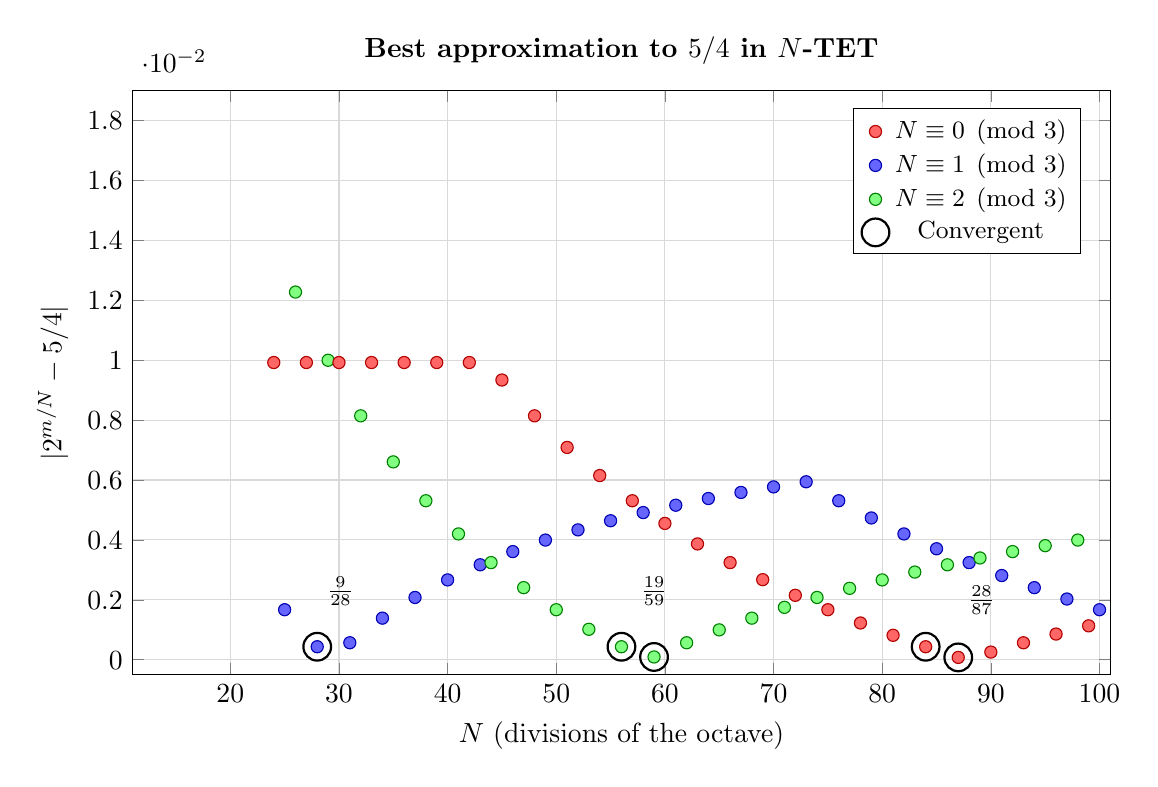
\begin{tikzpicture}
\begin{axis}[
    width=14cm, height=9cm,
    xlabel={$N$ (divisions of the octave)},
    ylabel={$|2^{m/N} - 5/4|$},
    title={\textbf{Best approximation to $5/4$ in $N$-TET}},
    xmin=11, xmax=101,
    ymin=-0.0005, ymax=0.019,
    grid=major,
    grid style={gray!30},
    legend pos=north east,
    legend style={font=\small},
    scatter/classes={
      a={mark=*,draw=red!70!black,fill=red!60,mark size=2.2pt},
      b={mark=*,draw=blue!70!black,fill=blue!60,mark size=2.2pt},
      c={mark=*,draw=green!50!black,fill=green!50,mark size=2.2pt}
    }
]
% Exact data: E(N) = |2^(round(N*alpha)/N) - 5/4|, alpha = log2(5/4)
% Color by N mod 3: a (red) = 0, b (blue) = 1, c (green) = 2
\addplot[scatter, only marks, scatter src=explicit symbolic]
coordinates {
(24, 0.009921) [a]
(25, 0.001669) [b]
(26, 0.012274) [c]
(27, 0.009921) [a]
(28, 0.000433) [b]
(29, 0.009996) [c]
(30, 0.009921) [a]
(31, 0.000566) [b]
(32, 0.008142) [c]
(33, 0.009921) [a]
(34, 0.001388) [b]
(35, 0.006604) [c]
(36, 0.009921) [a]
(37, 0.002078) [b]
(38, 0.005307) [c]
(39, 0.009921) [a]
(40, 0.002664) [b]
(41, 0.004199) [c]
(42, 0.009921) [a]
(43, 0.003169) [b]
(44, 0.003242) [c]
(45, 0.009337) [a]
(46, 0.003609) [b]
(47, 0.002406) [c]
(48, 0.008142) [a]
(49, 0.003994) [b]
(50, 0.001669) [c]
(51, 0.007087) [a]
(52, 0.004335) [b]
(53, 0.001016) [c]
(54, 0.006148) [a]
(55, 0.004639) [b]
(56, 0.000433) [c]
(57, 0.005307) [a]
(58, 0.004912) [b]
(59, 0.000092) [c]
(60, 0.004550) [a]
(61, 0.005158) [b]
(62, 0.000566) [c]
(63, 0.003865) [a]
(64, 0.005381) [b]
(65, 0.000996) [c]
(66, 0.003242) [a]
(67, 0.005584) [b]
(68, 0.001388) [c]
(69, 0.002672) [a]
(70, 0.005769) [b]
(71, 0.001748) [c]
(72, 0.002150) [a]
(73, 0.005940) [b]
(74, 0.002078) [c]
(75, 0.001669) [a]
(76, 0.005307) [b]
(77, 0.002383) [c]
(78, 0.001226) [a]
(79, 0.004732) [b]
(80, 0.002664) [c]
(81, 0.000815) [a]
(82, 0.004199) [b]
(83, 0.002926) [c]
(84, 0.000433) [a]
(85, 0.003704) [b]
(86, 0.003169) [c]
(87, 0.000077) [a]
(88, 0.003242) [b]
(89, 0.003396) [c]
(90, 0.000255) [a]
(91, 0.002810) [b]
(92, 0.003609) [c]
(93, 0.000566) [a]
(94, 0.002406) [b]
(95, 0.003807) [c]
(96, 0.000857) [a]
(97, 0.002026) [b]
(98, 0.003994) [c]
(99, 0.001131) [a]
(100, 0.001669) [b]
};

% Overlay: mark convergent denominators and their multiples
\addplot[only marks, mark=o, mark size=5pt, draw=black, thick]
coordinates {
(28, 0.000433) (56, 0.000433) (84, 0.000433) (59, 0.000092) (87, 0.000077)
};

% Legend entries via dummy plots
\addplot[only marks, mark=*, mark size=2.2pt, red!60, draw=red!70!black] coordinates {(-1,-1)};
\addlegendentry{$N \equiv 0\pmod{3}$}
\addplot[only marks, mark=*, mark size=2.2pt, blue!60, draw=blue!70!black] coordinates {(-1,-1)};
\addlegendentry{$N \equiv 1\pmod{3}$}
\addplot[only marks, mark=*, mark size=2.2pt, green!50, draw=green!50!black] coordinates {(-1,-1)};
\addlegendentry{$N \equiv 2\pmod{3}$}
\addplot[only marks, mark=o, mark size=4pt, draw=black, thick] coordinates {(-1,-1)};
\addlegendentry{Convergent}

% Annotations
\node[anchor=south west, font=\footnotesize] at (axis cs:28,0.0015) {$\frac{9}{28}$};
\node[anchor=south, font=\footnotesize] at (axis cs:59,0.0015) {$\frac{19}{59}$};
\node[anchor=south west, font=\footnotesize] at (axis cs:87,0.0012) {$\frac{28}{87}$};

\end{axis}
\end{tikzpicture}
\caption{Error in best approximation to the just major third
  ($5/4$) in $N$-TET, colored by $N \bmod 3$.
  Circled points are convergent denominators of~$\log_2(5/4)$.
  The three-strand structure arises because
  $\log_2(5/4) \approx 1/3$.}
\label{fig:strands}
\end{figure}

%==================================================================
\section{Summary}
\label{sec:summary}

The three-strand pattern in the equal temperament graph is not a
coincidence of music theory---it is a universal consequence of
Diophantine approximation near a low-order rational.  The same
mechanism, with $\log_2 3$ replacing $\log_2(5/4)$, governs the
cell-error structure of the Collatz torus sieve.  In both cases:

\begin{itemize}
\item The continued fraction of the irrational constant determines
  where the ``record'' approximations fall (convergent denominators).
\item The first convergent's denominator determines how many strands
  appear (here $3$, from $1/3$).
\item Lattice refinements that are multiples of existing denominators
  produce no improvement (the $N=24$ stagnation).
\item Baker-type lower bounds on linear forms in logarithms guarantee
  that the error can never vanish, creating the ``moat'' between strands.
\end{itemize}

\noindent
In the words of equal temperament: \emph{the twelve-tone scale cannot
perfectly tune the major third, because $\log_2 5$ is irrational and
its continued fraction traps every multiple of $12$ in the same
strand.}  In the words of the Collatz conjecture: \emph{the trajectory
cannot stagnate, because $\log_2 3$ is irrational and Baker's theorem
forces the deficit to grow.}

The graph is, in essence, a one-dimensional cross-section of the
two-dimensional torus sieve.

\bigskip\noindent
\textbf{Acknowledgment.}  The original question and graph are due to
a discussion on Substack.

\end{document}
